\documentclass[aspectratio=169,c]{beamer}
\usetheme{default}
\usecolortheme{dove}
\setbeamertemplate{navigation symbols}{}

% ── Fonts and microtypography ──────────────────────────────────
\usepackage{lmodern}
\usepackage{microtype}

% ── Color palette ──────────────────────────────────────────────
\definecolor{primary}{RGB}{23,63,95}
\definecolor{medgray}{RGB}{140,140,140}

\setbeamercolor{title}{fg=primary}
\setbeamercolor{subtitle}{fg=medgray}
\setbeamercolor{frametitle}{fg=primary}
\setbeamercolor{structure}{fg=primary}

% ── Frame titles (centered, colored) ──────────────────────────
\setbeamertemplate{frametitle}[default][center]

% ── Title page ─────────────────────────────────────────────────
\setbeamertemplate{title page}{
  \vfill
  \centering
  {\color{primary!40}\rule{0.45\textwidth}{0.4pt}}\\[1.5em]
  {\usebeamerfont{title}\usebeamercolor[fg]{title}\inserttitle}\\[0.8em]
  {\usebeamerfont{subtitle}\usebeamercolor[fg]{subtitle}\insertsubtitle}\\[1.5em]
  {\color{primary!40}\rule{0.45\textwidth}{0.4pt}}
  \vfill
}

% ── Footline ───────────────────────────────────────────────────
\newcommand{\defaultfootline}{%
  \setbeamertemplate{footline}{%
    \hfill{\color{medgray}\scriptsize\insertframenumber\kern14pt}\vskip6pt%
  }%
}
\defaultfootline

\newcommand{\hideframenumber}{%
  \setbeamertemplate{footline}{}%
  \addtocounter{framenumber}{-1}%
}
\newcommand{\showframenumber}{\defaultfootline}

% ── Section pages ────────────────────────────────────────────
\setbeamertemplate{section page}{
  \centering
  \vfill
  {\color{primary!40}\rule{0.35\textwidth}{0.4pt}}\\[1.2em]
  {\LARGE\bfseries\color{primary}\thesection.~\insertsection}\\[1.2em]
  {\color{primary!40}\rule{0.35\textwidth}{0.4pt}}
  \vfill
}

% ── Spacing ────────────────────────────────────────────────────
\setbeamertemplate{itemize/enumerate body begin}{\setlength\itemsep{6pt}}
\setbeamertemplate{itemize/enumerate subbody begin}{\setlength\itemsep{4pt}}
\renewcommand{\arraystretch}{1.25}

\setbeamertemplate{footline}[frame number]

% ==============================================================
\title{Matching-Based Control Groups}
\subtitle{Constructing Comparable Controls for Cyclone Impact Estimation}

\begin{document}

{\hideframenumber
\begin{frame}
\titlepage
\end{frame}
\showframenumber}

% ===============================================================
\section{Motivation}
% ===============================================================

{\hideframenumber
\begin{frame}
\sectionpage
\end{frame}
\showframenumber}

\begin{frame}{The Control Group Problem}
In TWFE local projections, the year FE absorbs the \textbf{average GDP path} across all countries:
\[
  \hat{\delta}_t \;\approx\; \frac{1}{N}\sum_{i=1}^{N}\bigl(y_{i,t+h} - y_{i,t-1} - \hat{\gamma}'X_{it}\bigr)
\]

\begin{itemize}
  \item \textbf{142 of 182} countries never experience a p95 cyclone shock
  \item These never-treated countries \textbf{dominate} the year FE $\to$ they define the counterfactual
  \item Never-treated concentrated in \textbf{Europe} (23) and \textbf{Africa} (38)
  \item Treated concentrated in \textbf{Americas} (12) and \textbf{Asia} (14)
  \item Region$\times$year FE eliminate the divergence, but can \emph{matching} achieve the same?
\end{itemize}
\end{frame}

\begin{frame}{Covariate Imbalance: Distributions}
\centering

\includegraphics[width=0.82\textwidth,height=0.68\textheight,keepaspectratio]{figures/covariate_imbalance.png}

\smallskip
\small
Pre-1990 means. Treated countries are poorer on average, more populous, and concentrated in different regions. Human capital is comparable.
\end{frame}

\begin{frame}{Covariate Imbalance: Standardized Differences}
\centering
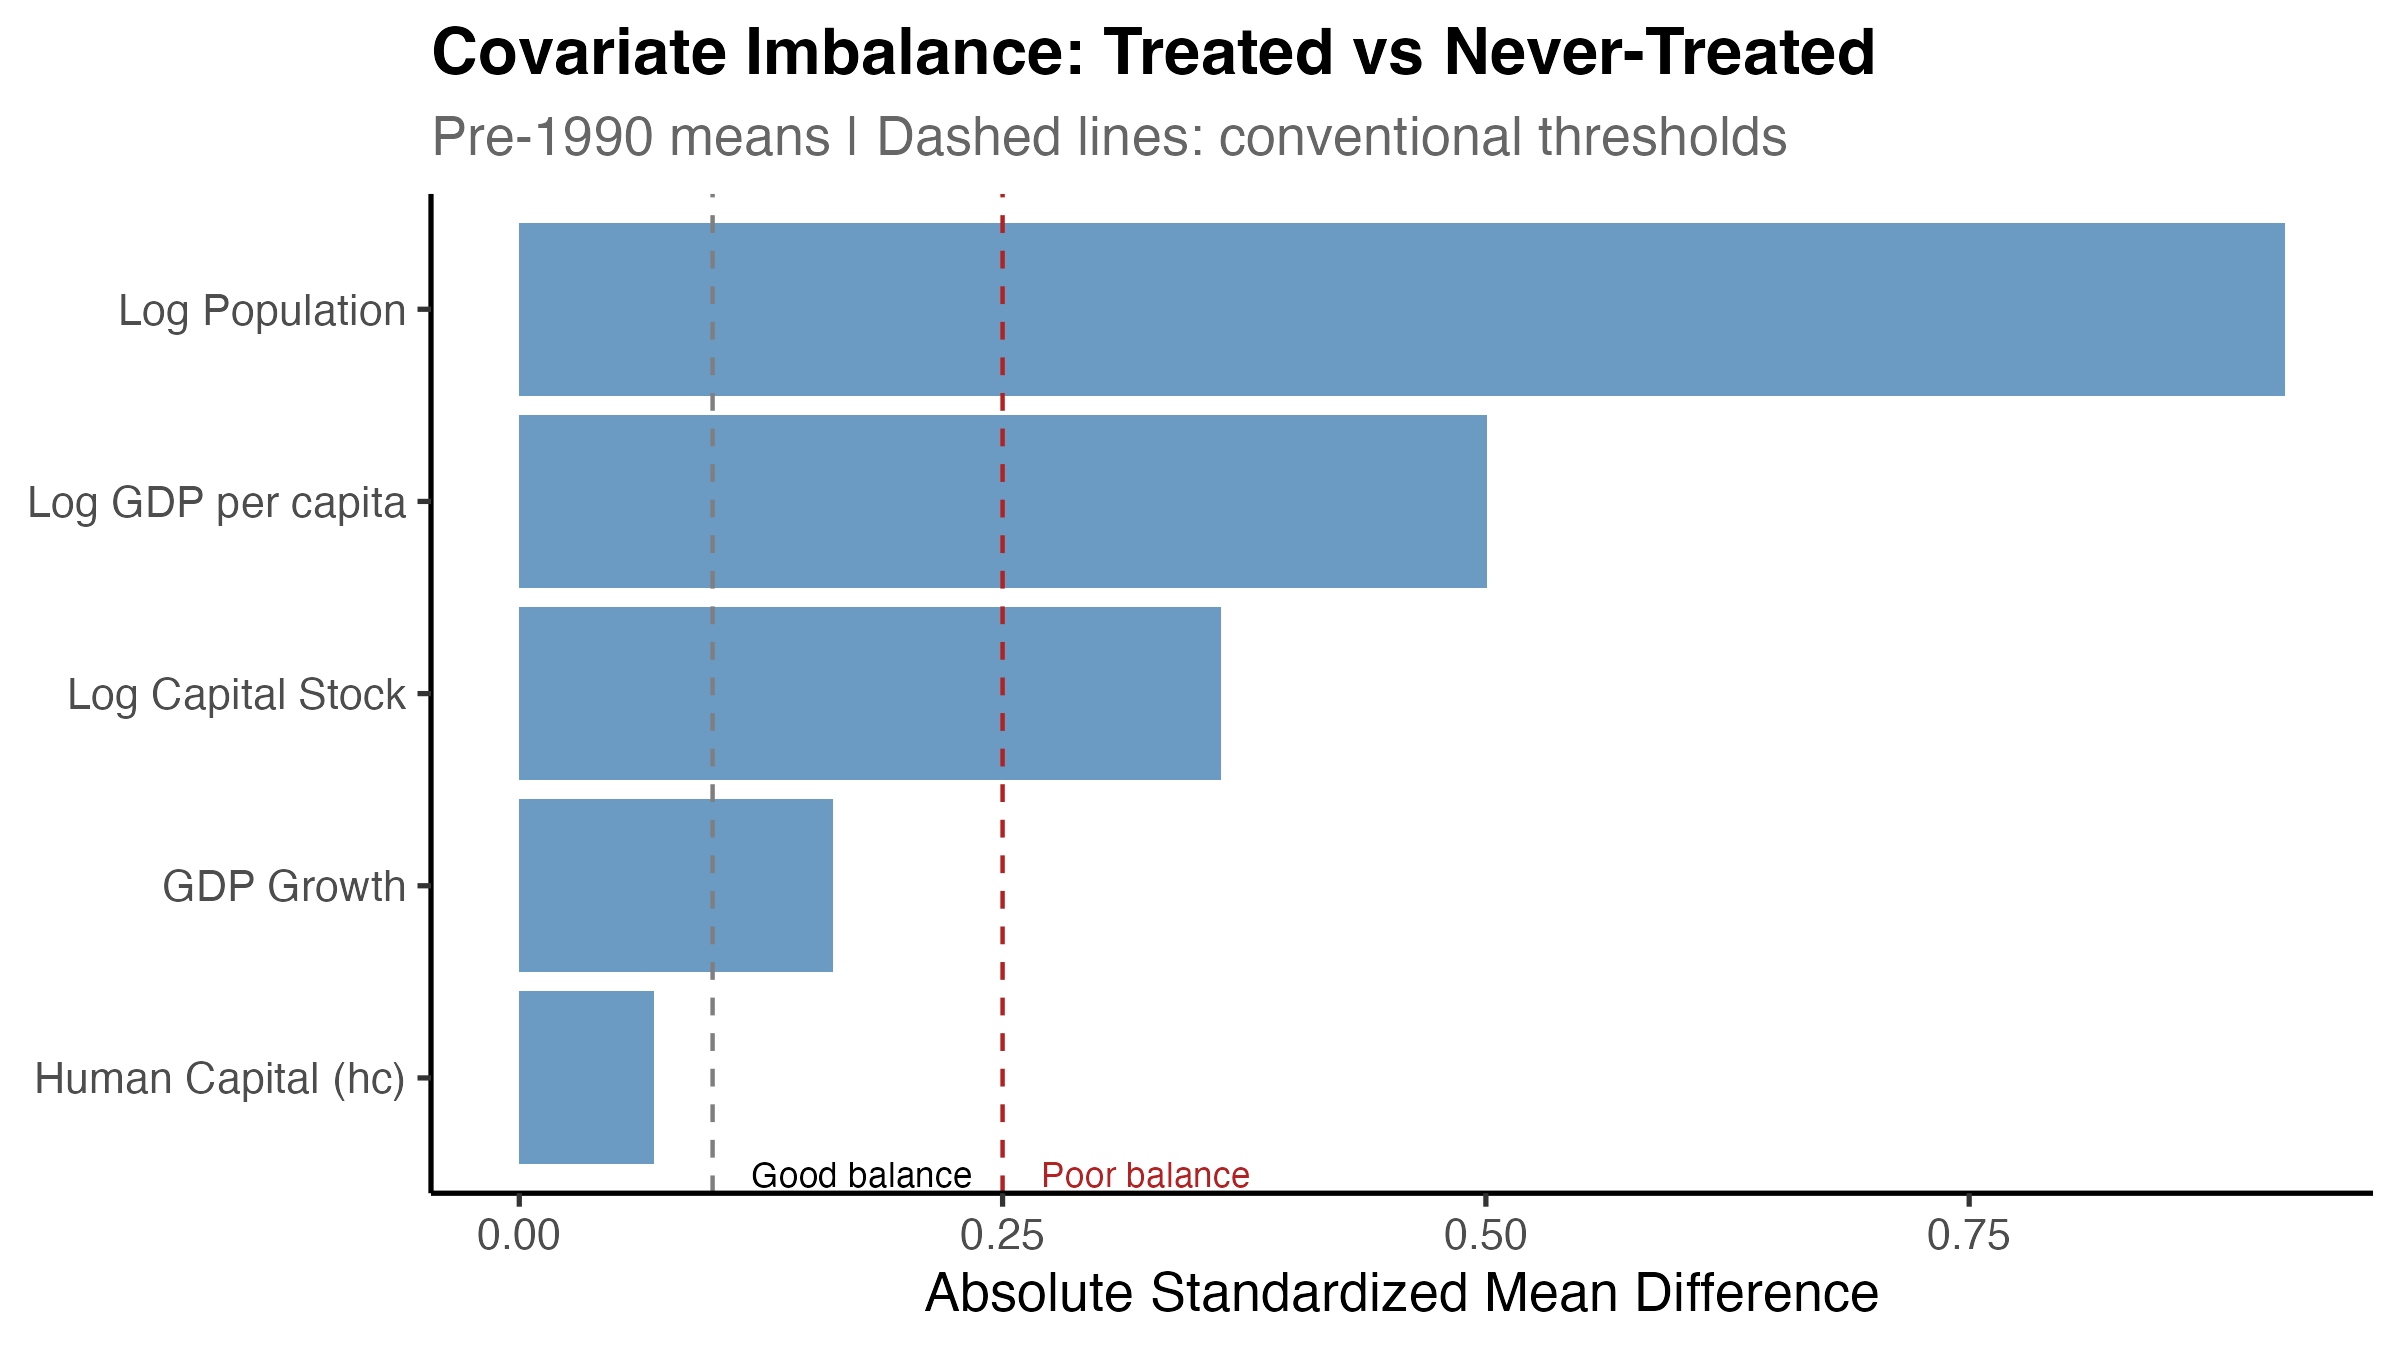
\includegraphics[width=0.75\textwidth,height=0.60\textheight,keepaspectratio]{figures/smd_before_matching.png}

\smallskip
\small
Population ($|$SMD$| = 0.91$) and log GDP per capita ($|$SMD$| = 0.50$) are far above the 0.25 threshold for acceptable balance. GDP growth and human capital are better balanced.
\end{frame}

% ===============================================================
\section{Matching Methods}
% ===============================================================

{\hideframenumber
\begin{frame}
\sectionpage
\end{frame}
\showframenumber}

\begin{frame}{Design}
\textbf{Matching unit}: Country (not country-year)
\begin{itemize}
  \item Match each ever-treated country to similar never-treated countries based on pre-1990 characteristics
  \item Covariates: mean log GDP pc, GDP growth, human capital (\texttt{hc}), log population, continent
  \item Re-run the period-interacted LP on the matched sample
\end{itemize}

\medskip
\textbf{Three methods} (all via \texttt{MatchIt}):
\begin{enumerate}
  \item \textbf{Propensity Score Matching} --- Nearest-neighbor on P(treated), ratio=2, caliper=0.25
  \item \textbf{Coarsened Exact Matching} --- Binned GDP and human capital $\times$ continent
  \item \textbf{Mahalanobis Distance} --- Multivariate distance, exact match on continent
\end{enumerate}

\medskip
\textbf{LP specification}: Same as main analysis --- \texttt{maxwind\_95}, period interaction, country polynomials + year FE
\end{frame}

\begin{frame}{Propensity Score Matching}
\centering
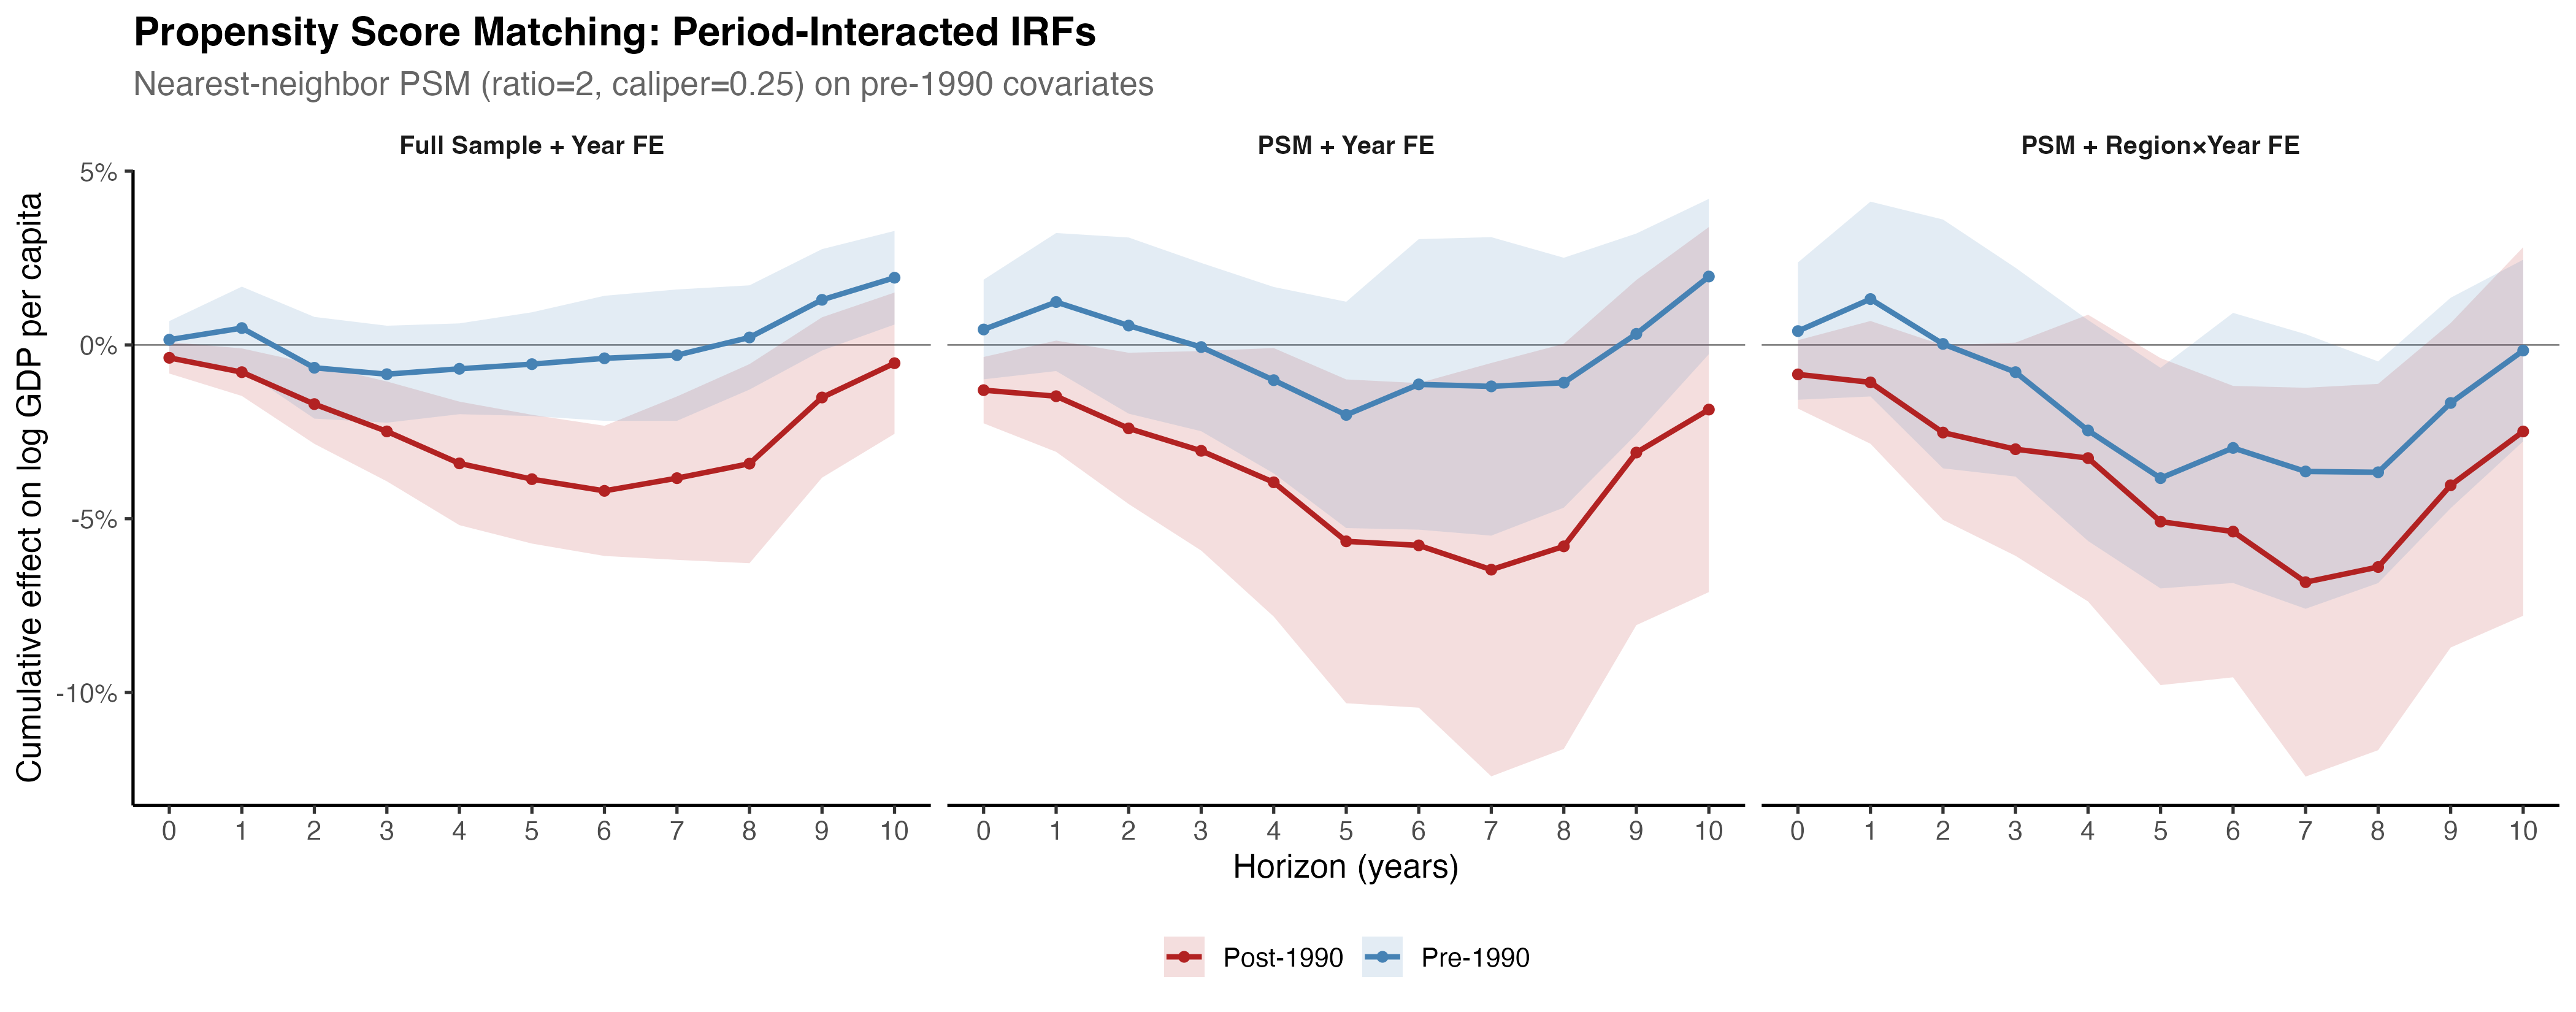
\includegraphics[width=\textwidth,height=0.62\textheight,keepaspectratio]{figures/irf_psm.png}

\smallskip
\small
PSM (ratio=2, caliper=0.25) matched 15 treated to 20 control countries. The caliper discards 17/32 treated countries with no good match, yielding a small sample. The post-pre gap ($-3.64$ pp) is similar to the full sample ($-3.31$ pp).
\end{frame}

\begin{frame}{Coarsened Exact Matching}
\centering

\includegraphics[width=\textwidth,height=0.62\textheight,keepaspectratio]{figures/irf_cem.png}

\smallskip
\small
CEM on binned GDP, human capital, and continent matched 25 treated to 54 control countries. The post-pre gap \textbf{shrinks from $-3.31$ to $-1.20$ pp} --- a 64\% reduction. CEM ensures covariate overlap within bins, directly addressing the composition problem.
\end{frame}

\begin{frame}{Mahalanobis Distance Matching}
\centering
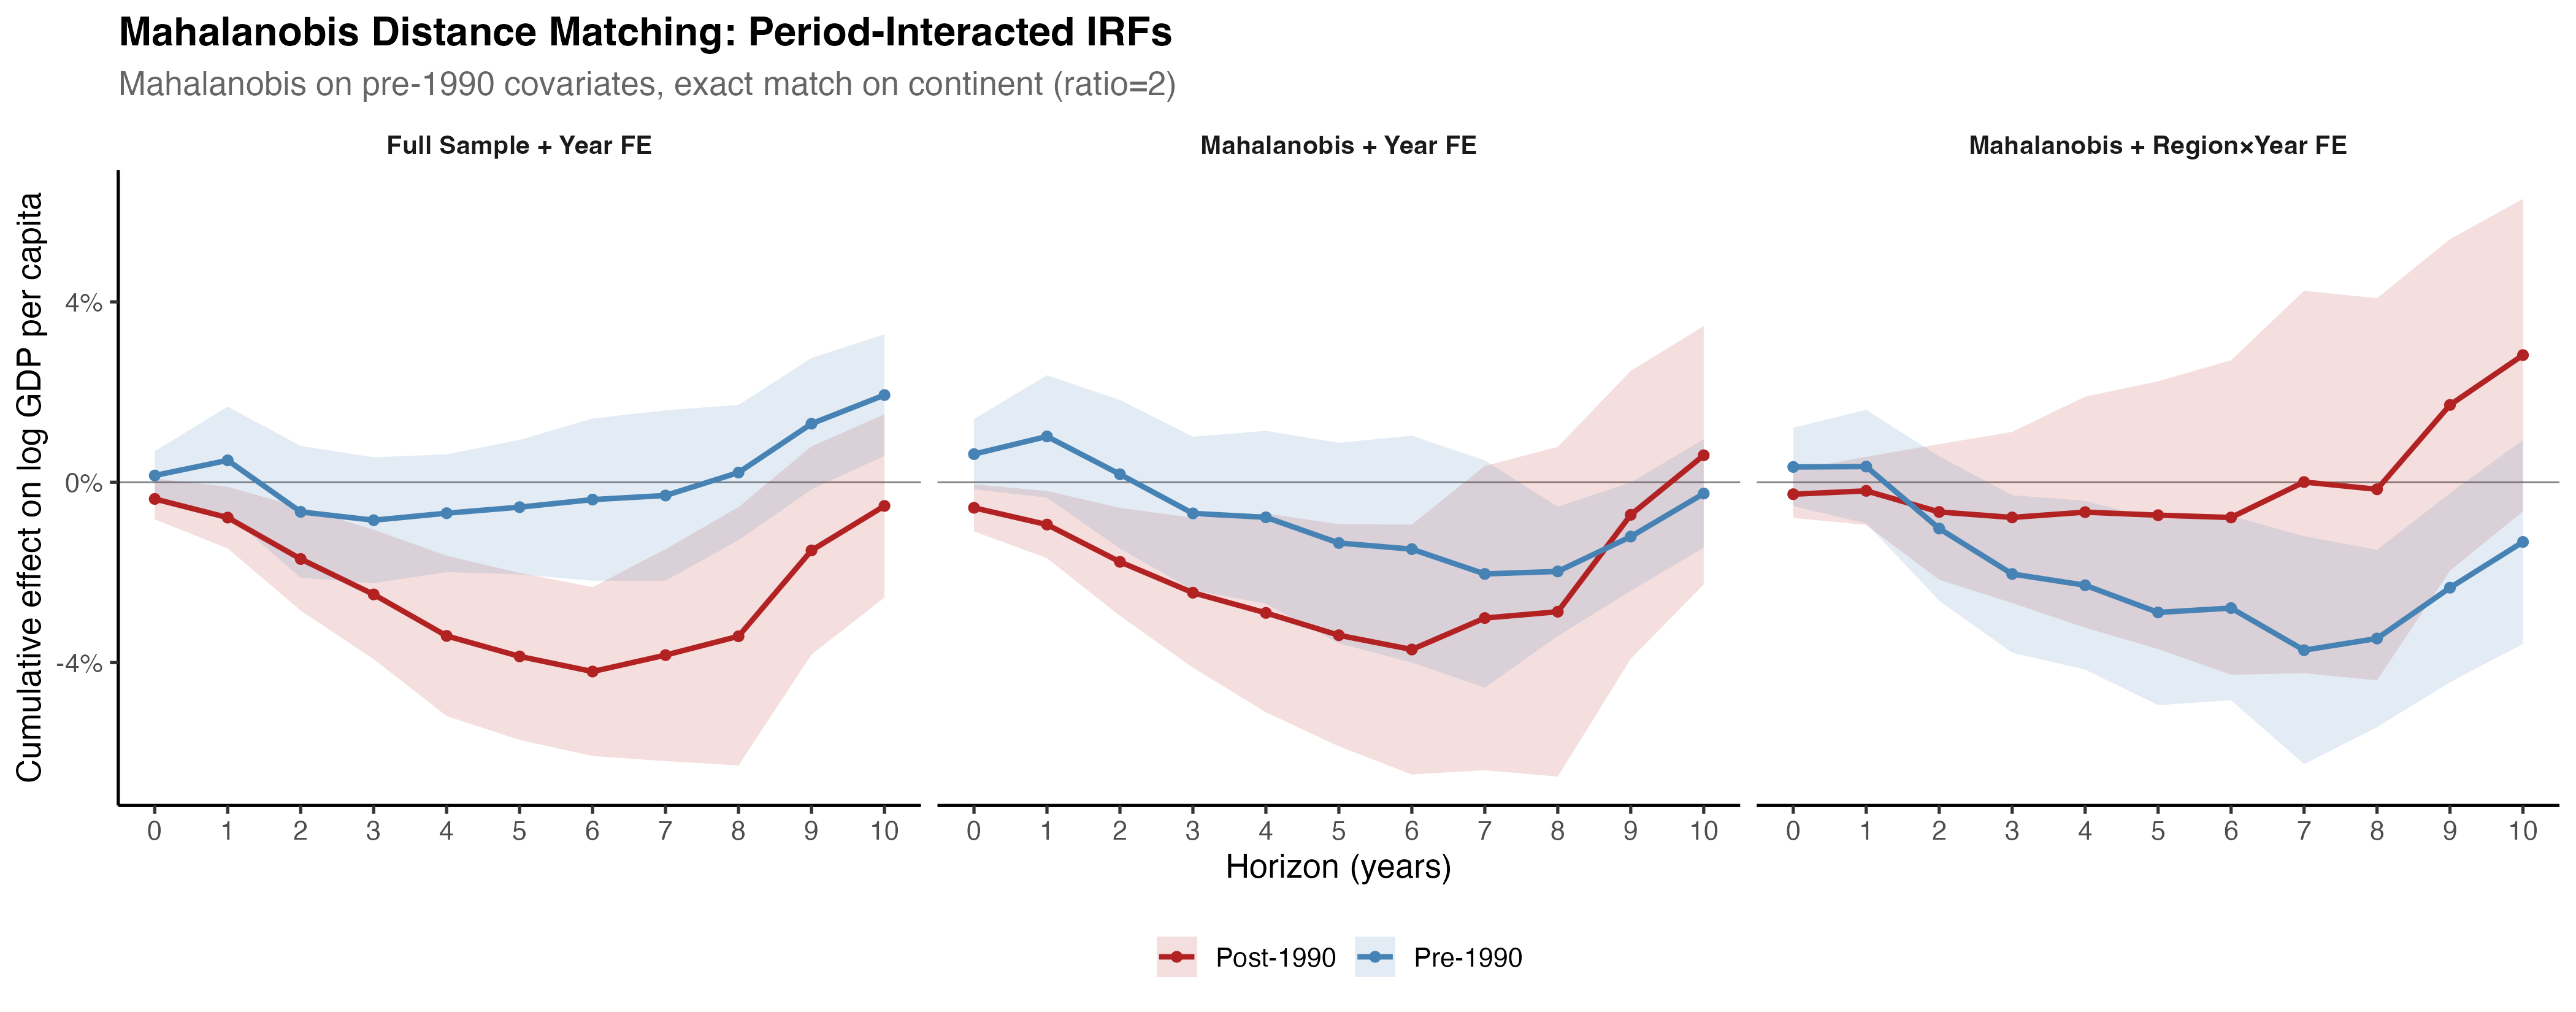
\includegraphics[width=\textwidth,height=0.62\textheight,keepaspectratio]{figures/irf_mahal.png}

\smallskip
\small
Mahalanobis matching with exact continent match retained 31 treated and 44 control countries. The gap reduces to $-2.05$ pp. Balance improvement is limited because some continents have very few controls (Europe: 23 controls for 1 treated; Oceania: 1 for 2).
\end{frame}

% ===============================================================
\section{Comparison}
% ===============================================================

{\hideframenumber
\begin{frame}
\sectionpage
\end{frame}
\showframenumber}

\begin{frame}{Balance Improvement Across Methods}
\centering
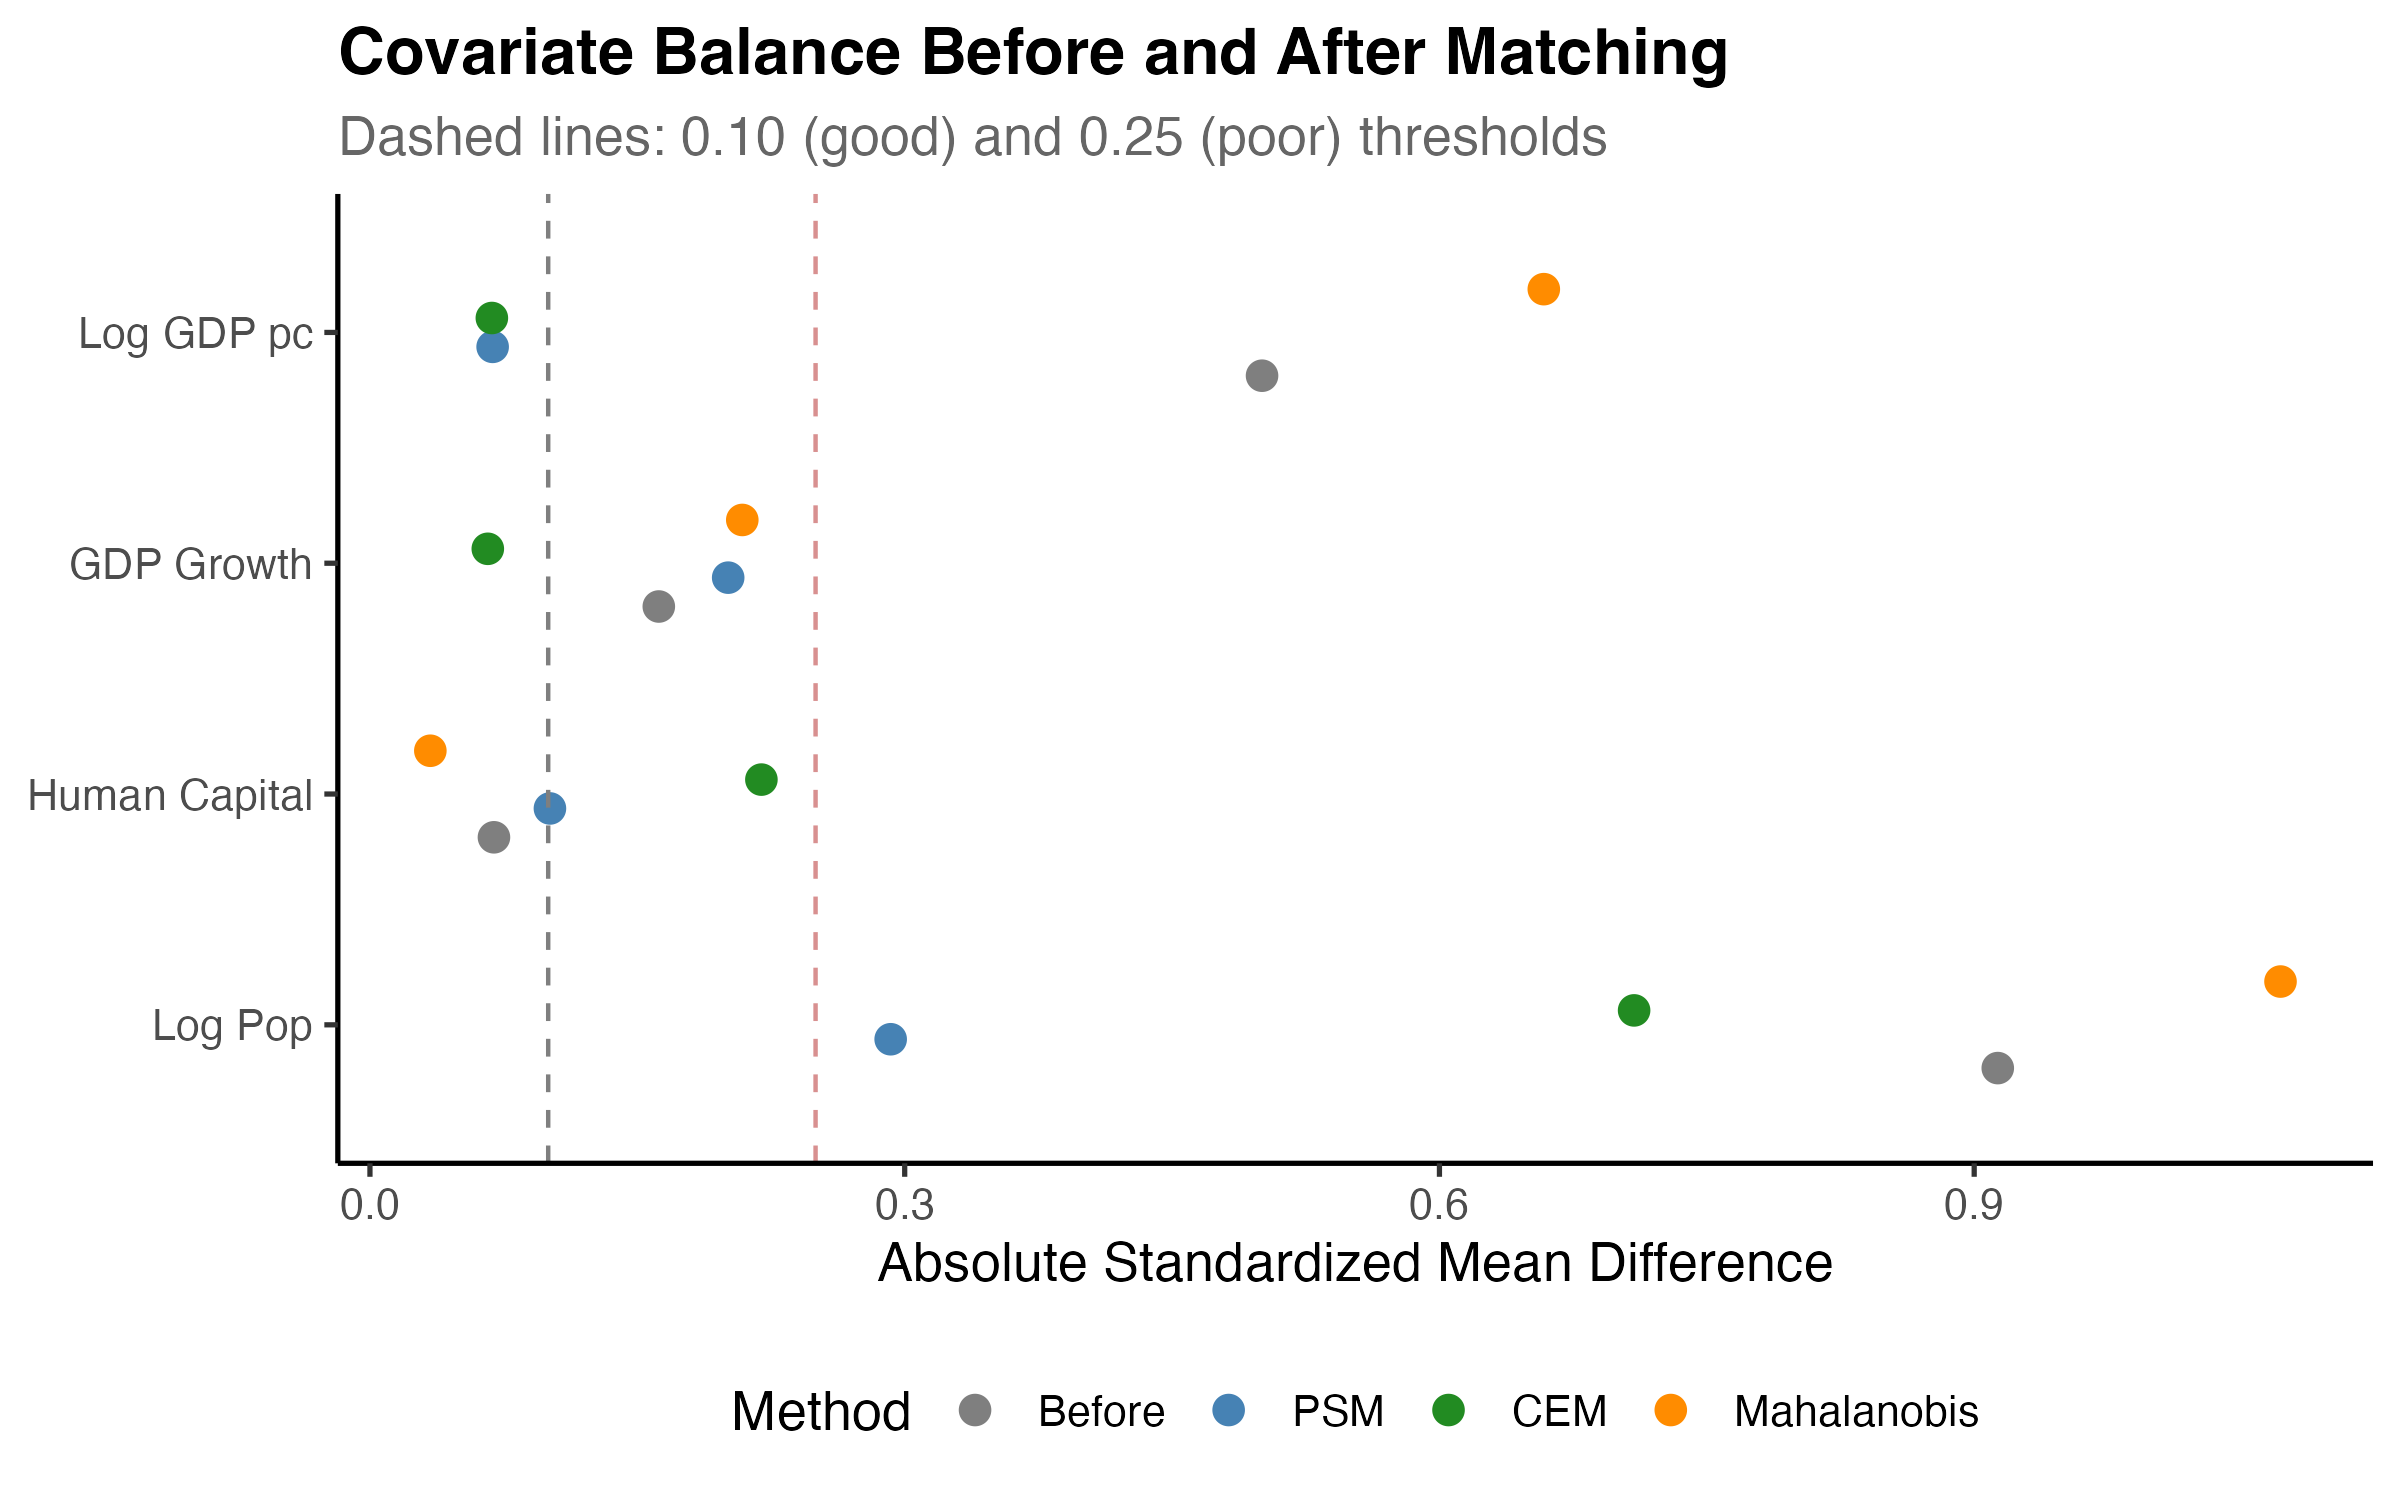
\includegraphics[width=0.78\textwidth,height=0.62\textheight,keepaspectratio]{figures/balance_improvement.png}

\smallskip
\small
CEM achieves the best balance on log GDP per capita and GDP growth. PSM improves GDP and population but worsens human capital slightly. Mahalanobis with exact continent match is constrained by sparse overlap.
\end{frame}

\begin{frame}{IRF Comparison: All Methods}
\centering
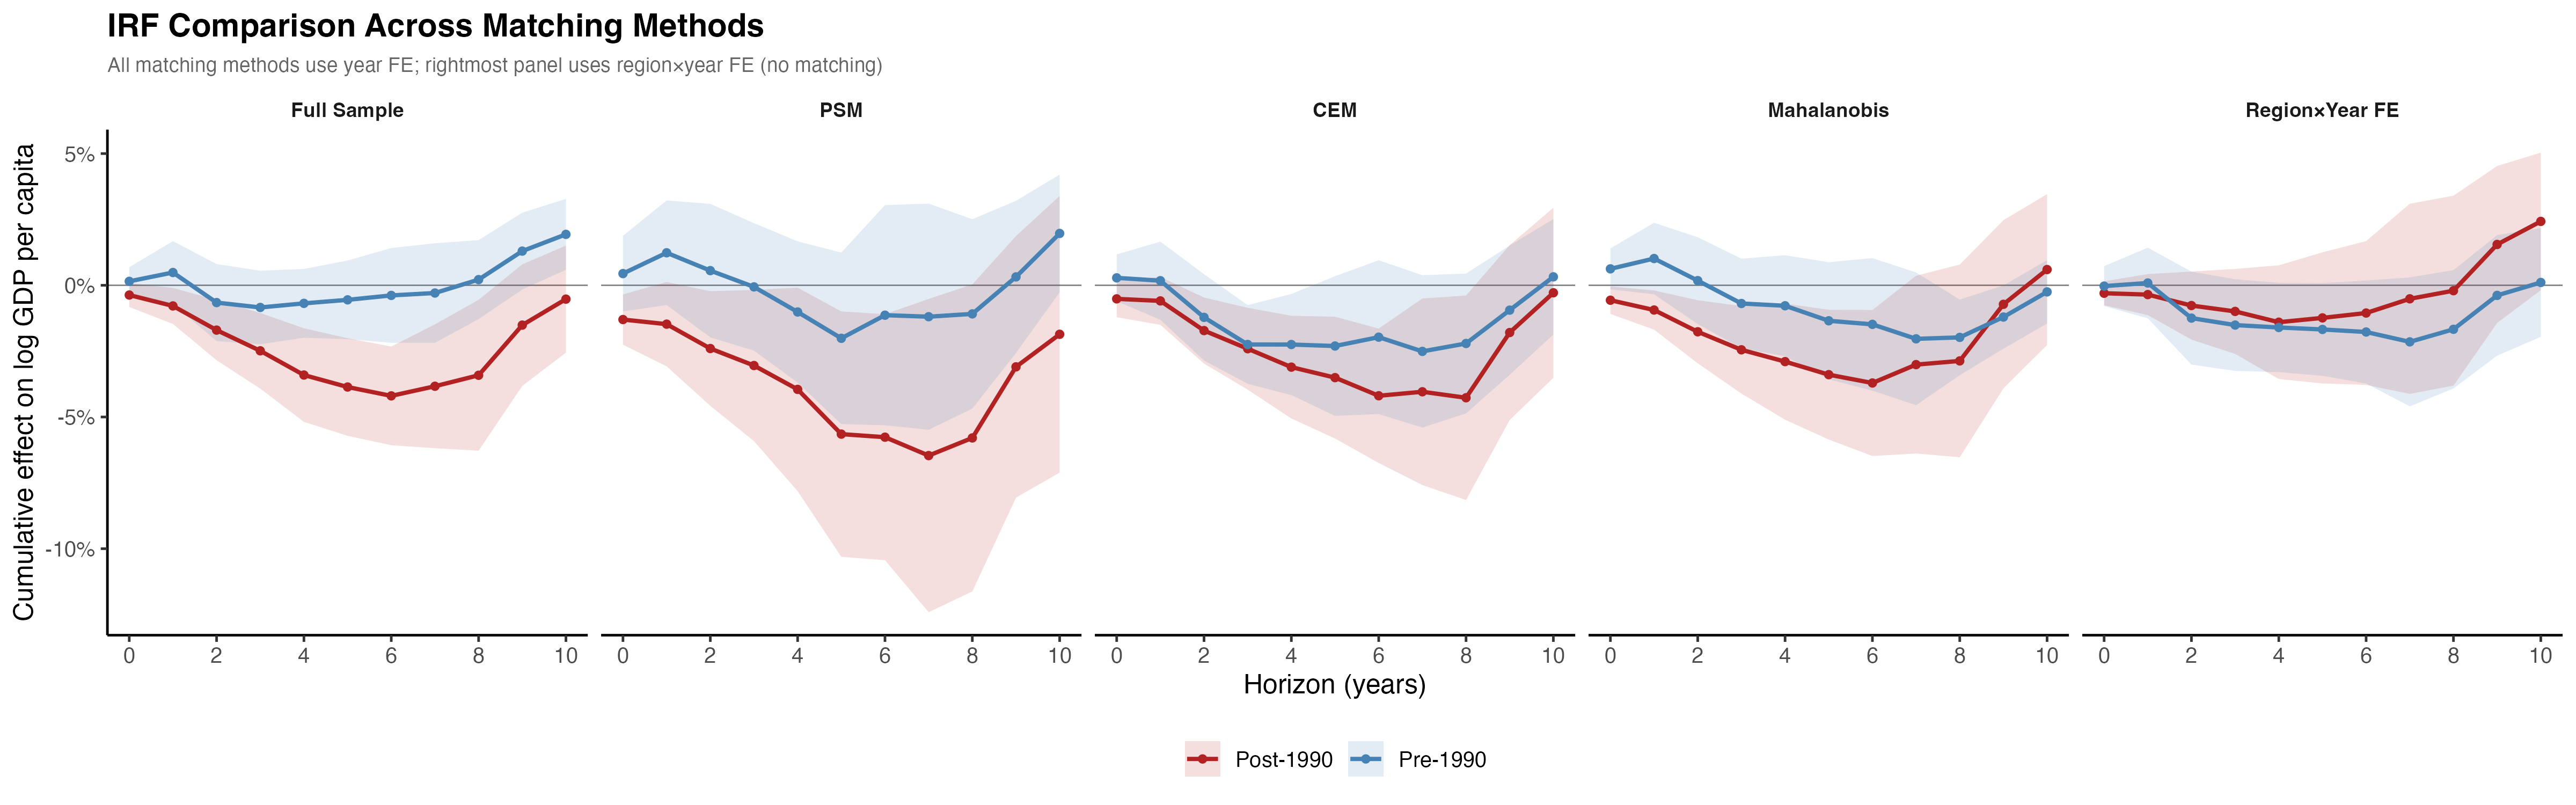
\includegraphics[width=\textwidth,height=0.58\textheight,keepaspectratio]{figures/irf_matching_comparison.png}

\smallskip
\small
Post-pre gap at $h = 5$: Full sample $= -3.31$ pp; PSM $= -3.64$ pp; CEM $= -1.20$ pp; Mahalanobis $= -2.05$ pp; Region$\times$Year FE $= +0.44$ pp. CEM reduces the gap most effectively among matching methods.
\end{frame}

\begin{frame}{Summary of Post-Pre Gaps at $h = 5$}
\centering
\begin{tabular}{l r r r}
\hline
\textbf{Method} & \textbf{Pre-1990} & \textbf{Post-1990} & \textbf{Gap (pp)} \\
\hline
Full Sample + Year FE       & $-0.6\%$  & $-3.9\%$  & $-3.31$ \\
PSM + Year FE               & $-2.0\%$  & $-5.7\%$  & $-3.64$ \\
CEM + Year FE               & $-2.3\%$  & $-3.5\%$  & $-1.20$ \\
Mahalanobis + Year FE       & $-1.3\%$  & $-3.4\%$  & $-2.05$ \\
Region$\times$Year FE       & $-1.7\%$  & $-1.2\%$  & $+0.44$ \\
\hline
\end{tabular}

\bigskip
\begin{itemize}
  \item CEM reduces the gap by 64\%, confirming the control group composition mechanism
  \item Matching improves the control group but does not fully resolve the problem
  \item Region$\times$year FE remain the most effective solution --- they absorb heterogeneous trends directly rather than selecting on observables
\end{itemize}
\end{frame}

\begin{frame}{Takeaways}
\begin{enumerate}
  \item \textbf{Matching confirms the diagnosis}: The post-pre divergence is driven by control group composition, not by a real change in cyclone impacts
  \medskip
  \item \textbf{CEM performs best} among matching methods: binning on GDP, human capital, and continent ensures comparable controls
  \medskip
  \item \textbf{PSM is limited}: The caliper discards too many treated countries (17/32), and the remaining matched sample still shows the full gap
  \medskip
  \item \textbf{Region$\times$year FE dominate}: They address the problem more directly by allowing different time trends per region, without losing sample size
  \medskip
  \item \textbf{Complementary evidence}: Matching and region$\times$year FE point to the same mechanism --- the matching results provide independent confirmation
\end{enumerate}
\end{frame}

\end{document}
